\subsection{Task 5 --- Experimenting with the SameSite Cokkie Method}
%
\begin{figure}
    \centering
    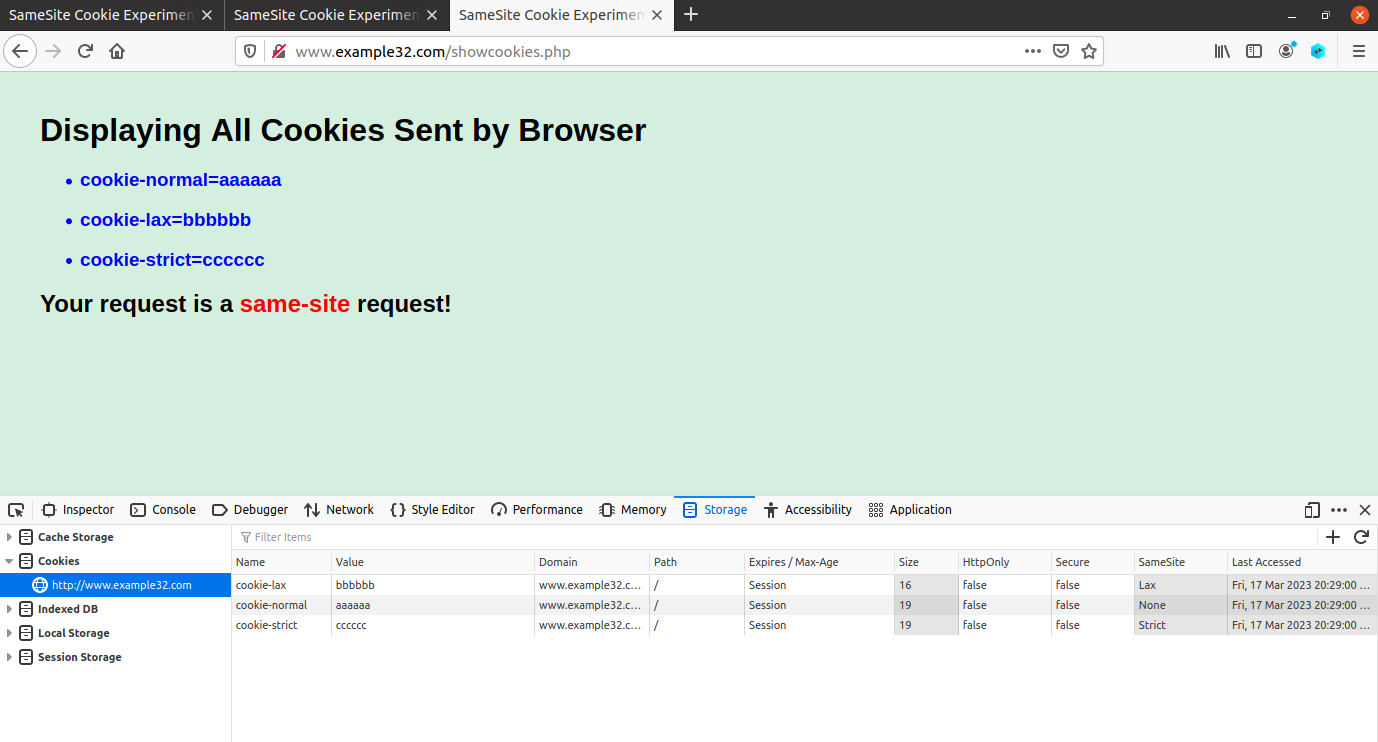
\includegraphics[height=\textheight,width=\textwidth,keepaspectratio]
    {figures/samesite_cookie_same.png}
    \caption{All cookies are sent within the same site.}
    \label{fig:samesite_cookie}
\end{figure}

\begin{figure}
    \centering
    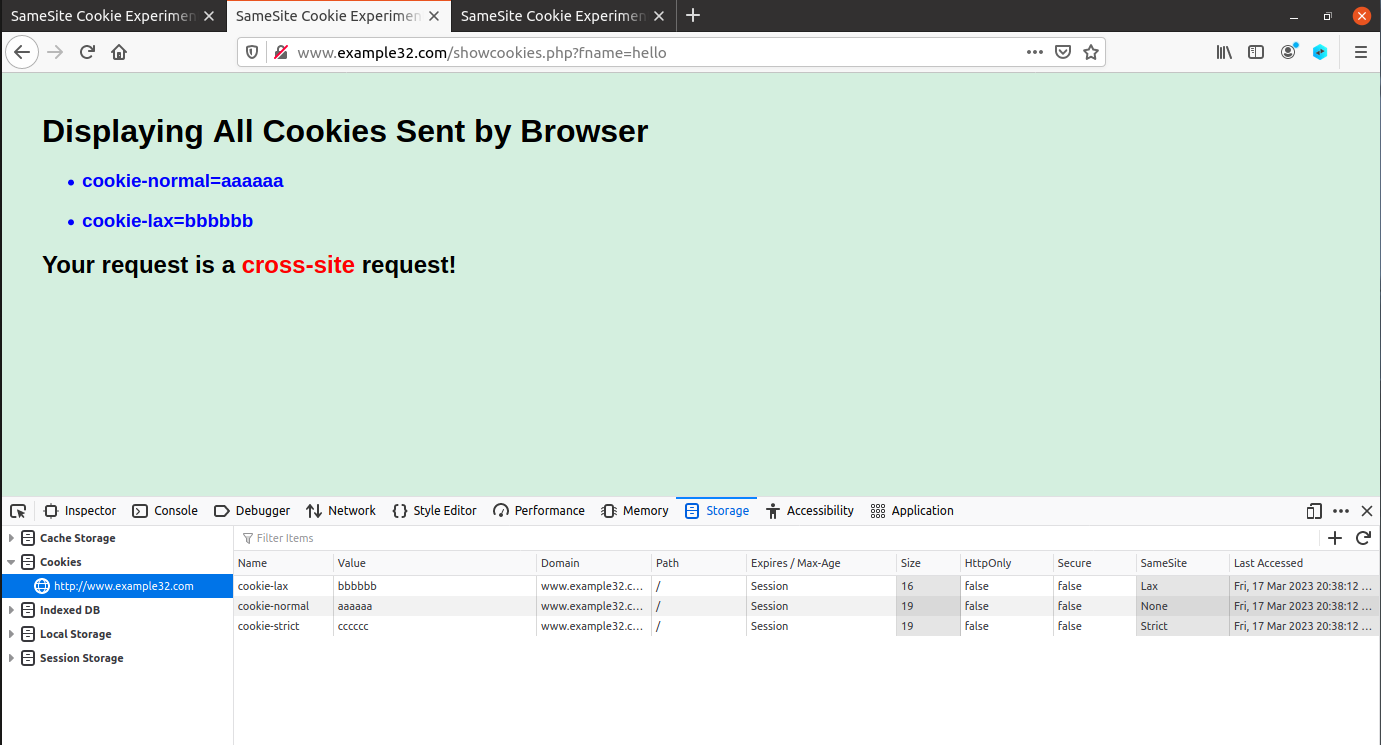
\includegraphics[height=\textheight,width=\textwidth,keepaspectratio]
    {figures/samesite_cookie_get_crosssite.png}
    \caption{The strict cookie is missing if a HTTP GET request is sent
    from a different site.}
    \label{fig:crosssite_cookie_get}
\end{figure}

\begin{figure}
    \centering
    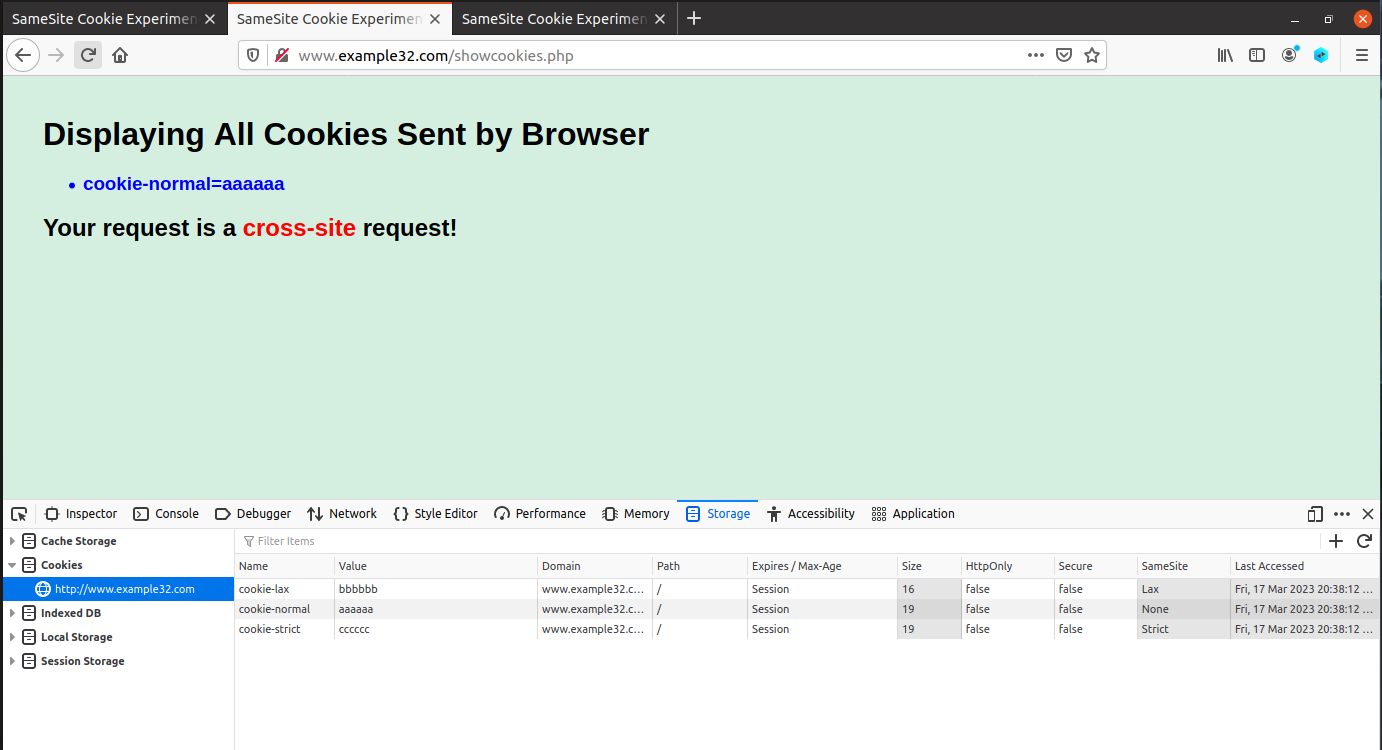
\includegraphics[height=\textheight,width=\textwidth,keepaspectratio]
    {figures/samesite_cookie_post_crosssite.png}
    \caption{Both strict and lax cookies are missing if a HTTP POST request
    is sent from a different site.}
    \label{fig:crosssite_cookie_post}
\end{figure}

We show here some definition of value of {\fontfamily{qcr}\selectfont SameSite}
attribute:

\begin{itemize}
    \item None: cookie can be sent in all contexts.
    \item Lax: besides the first-party site (the site that is in the same domain
    with the origin), cookie only can be sent to the third-party site (the site that
    is in a different domain from the origin) through top-level GET requests.
    \item Strict: cookie only can be sent to the first-party site. In other words,
    cookie only is sent within a specific domain.
\end{itemize}

After playing with two experiment pages, we obtained some observations.
Both cases of sending a HTTP GET and HTTP POST request from {\fontfamily{qcr}
\selectfont www.example32.com/testing.html}, all cookies are sent (see \autoref{fig:samesite_cookie}).
The reason is that the site we were sending the request from is in the same domain
with the destination site (both are in {\fontfamily{qcr}\selectfont www.example32.com}).
On the other hand, on the experiments with {\fontfamily{qcr}\selectfont
www.attacker32.com/testing.html}, when we sent a HTTP GET request, the {\fontfamily{qcr}\selectfont cookie-strict}
was missing (only {\fontfamily{qcr}\selectfont cookie-normal} and {\fontfamily{qcr}\selectfont cookie-lax}
were sent, see \autoref{fig:crosssite_cookie_get}).
The reason is that the {\fontfamily{qcr}\selectfont cookie-strict} only can be sent within
the first-party site, while the {\fontfamily{qcr}\selectfont cookie-lax} can be sent to
the third-party site  through top-level GET
requests. In addtion, {\fontfamily{qcr}\selectfont cookie-normal} can be sent in all contexts.
In the case of sending a HTTP POST request, only {\fontfamily{qcr}\selectfont cookie-normal}
can be sent (see \autoref{fig:crosssite_cookie_post}). In this case, {\fontfamily{qcr}\selectfont
cookie-lax} even cannot be sent as the type of the request is POST, while a lax cookie can only
be sent over a top-level GET request.

As each cookie has its own {\fontfamily{qcr}\selectfont domain} field which contains the domain
of the original site creating it. Once the SameSite attribute is defined, the server can compare
the value of {\fontfamily{qcr}\selectfont domain} field of each cookie and the site are being
requested to detect wheather a request is a cross-site or same-site request.

As shown in above CSRF attacks, some key values are embedded in URL or HTTP request body
such as {\fontfamily{qcr}\selectfont guid,name,friend, etc.}. These values
are easily hard-coded by the attacker, and without secret tokens, CSRF attacks
are simply conducted. To solve this problem, Elgg should store those key values
as a cookie and set attribute {\fontfamily{qcr}\selectfont SameSite=strict}.
For example, the server can set Alice's user id as a cookie in {\fontfamily{qcr}\selectfont
Set-Cookie} header like this:

\begin{verbatim}
    Set-Cookie: guid=56; SameSite=strict
\end{verbatim}

By setting strict SameSite cookie, the stored values are only sent to sites that are
in the same domain with the origin, preventing CSRF attacks.